\documentclass[12pt]{article}
\usepackage{geometry}                % See geometry.pdf to learn the layout options. There are lots.
\geometry{letterpaper}                   % ... or a4paper or a5paper or ... 
\usepackage{graphicx}
\usepackage{amssymb}
\usepackage{amsthm}
\usepackage{epstopdf}
\usepackage[utf8]{inputenc}
\usepackage[usenames,dvipsnames]{color}
\usepackage[table]{xcolor}
\usepackage{hyperref}
\DeclareGraphicsRule{.tif}{png}{.png}{`convert #1 `dirname #1`/`basename #1 .tif`.png}

\theoremstyle{definition}
\newtheorem{example}{Example}

\newcommand{\projectname}{Allround Manager}
\newcommand{\productname}{Allround Manager}
\newcommand{\projectleader}{Christian Bachl}
\newcommand{\documentstatus}{In process}
%\newcommand{\documentstatus}{Submitted}
%\newcommand{\documentstatus}{Released}
\newcommand{\version}{V. 1.0}

\begin{document}
\begin{titlepage}
\begin{flushright}
%\includegraphics[scale=.5]{htlleondinglogo.png}\\
\end{flushright}

\vspace{10em}

\begin{center}
{\Huge System Specification} \\[3em]
{\LARGE \productname} \\[3em]
\end{center}

\begin{flushleft}
\begin{tabular}{|l|l|}
\hline
Project Name & \projectname \\ \hline
Project Leader & \projectleader \\ \hline
Document state & \documentstatus \\ \hline
Version & \version \\ \hline
\end{tabular}
\end{flushleft}

\end{titlepage}
\section*{Revisions}
\begin{tabular}{|l|l|l|}
\hline
\cellcolor[gray]{0.5}\textcolor{white}{Date} & \cellcolor[gray]{0.5}\textcolor{white}{Author} & \cellcolor[gray]{0.5}\textcolor{white}{Change} \\ \hline
November 29, 2018&C. Christian/Jusic version \\ \hline
\end{tabular}
\pagebreak

\tableofcontents
\pagebreak

\section{Initial Situation and Goal}

\subsection{Initial Situation}
Organizing an event involves a lot of organizational steps for the event leader. A non-exhaustive list of tasks could be
\begin{itemize}
\item When the event involves some trip a generally accepted destination has to be aligned
\item Send invitations to all participants
\item Keeping track of registrations or de-registration of participants
\item Gathering information about the participants like home addresses, passport numbers, etc.
\item Provisioning of information about the event for the participants, like the aim of the event, agenda, other participants, etc.
\item bills of outstanding services like a prepayment for an event.
\end{itemize}

Currently, a wide variety of tools has to be used to accomplish the above-mentioned tasks.
\begin{itemize}
\item Most of the communication is done via WhatsApp or similar social media apps.
\item Lists of participants, their status, etc. are organized via spreadsheets
\item Outstanding bills must be paid with a payment slip or in cash.
\end{itemize}


The combination of different tools and a very decentralized way of organization makes it hard for the event organizer to stay on top of the things. More often than not these events struggle with late minute change or an announcement.  This could be:
\begin{itemize}
\item meeting point of the event/journey.
\item A date where the event takes place.
\end{itemize}


Doing these things may cause some troubles for the event organizer, like:

\begin{itemize}
\item when you have a lot of participants you may forget somebody
\item When billing, for example, participants want to pay only from the location where they have entered.
\item the leader must be every time available like: user wants to de-register or want to know many participants take part in the event.
\item getting spammed by registrations in WhatsApp.  
\end{itemize}


\subsubsection{Application Domain}



\subsubsection{Glossary}

\subsubsection{Model of the Application Domain}

\subsection{Goal Definition}
The main goal is to create a software to speed up and simplify the process of organizing an event. We especially want to make it possible for people who don't have the opportunity to afford expansive software or an event manager.
\pagebreak

\section{Functional Requirements}

\subsection{Use Case Join Event}

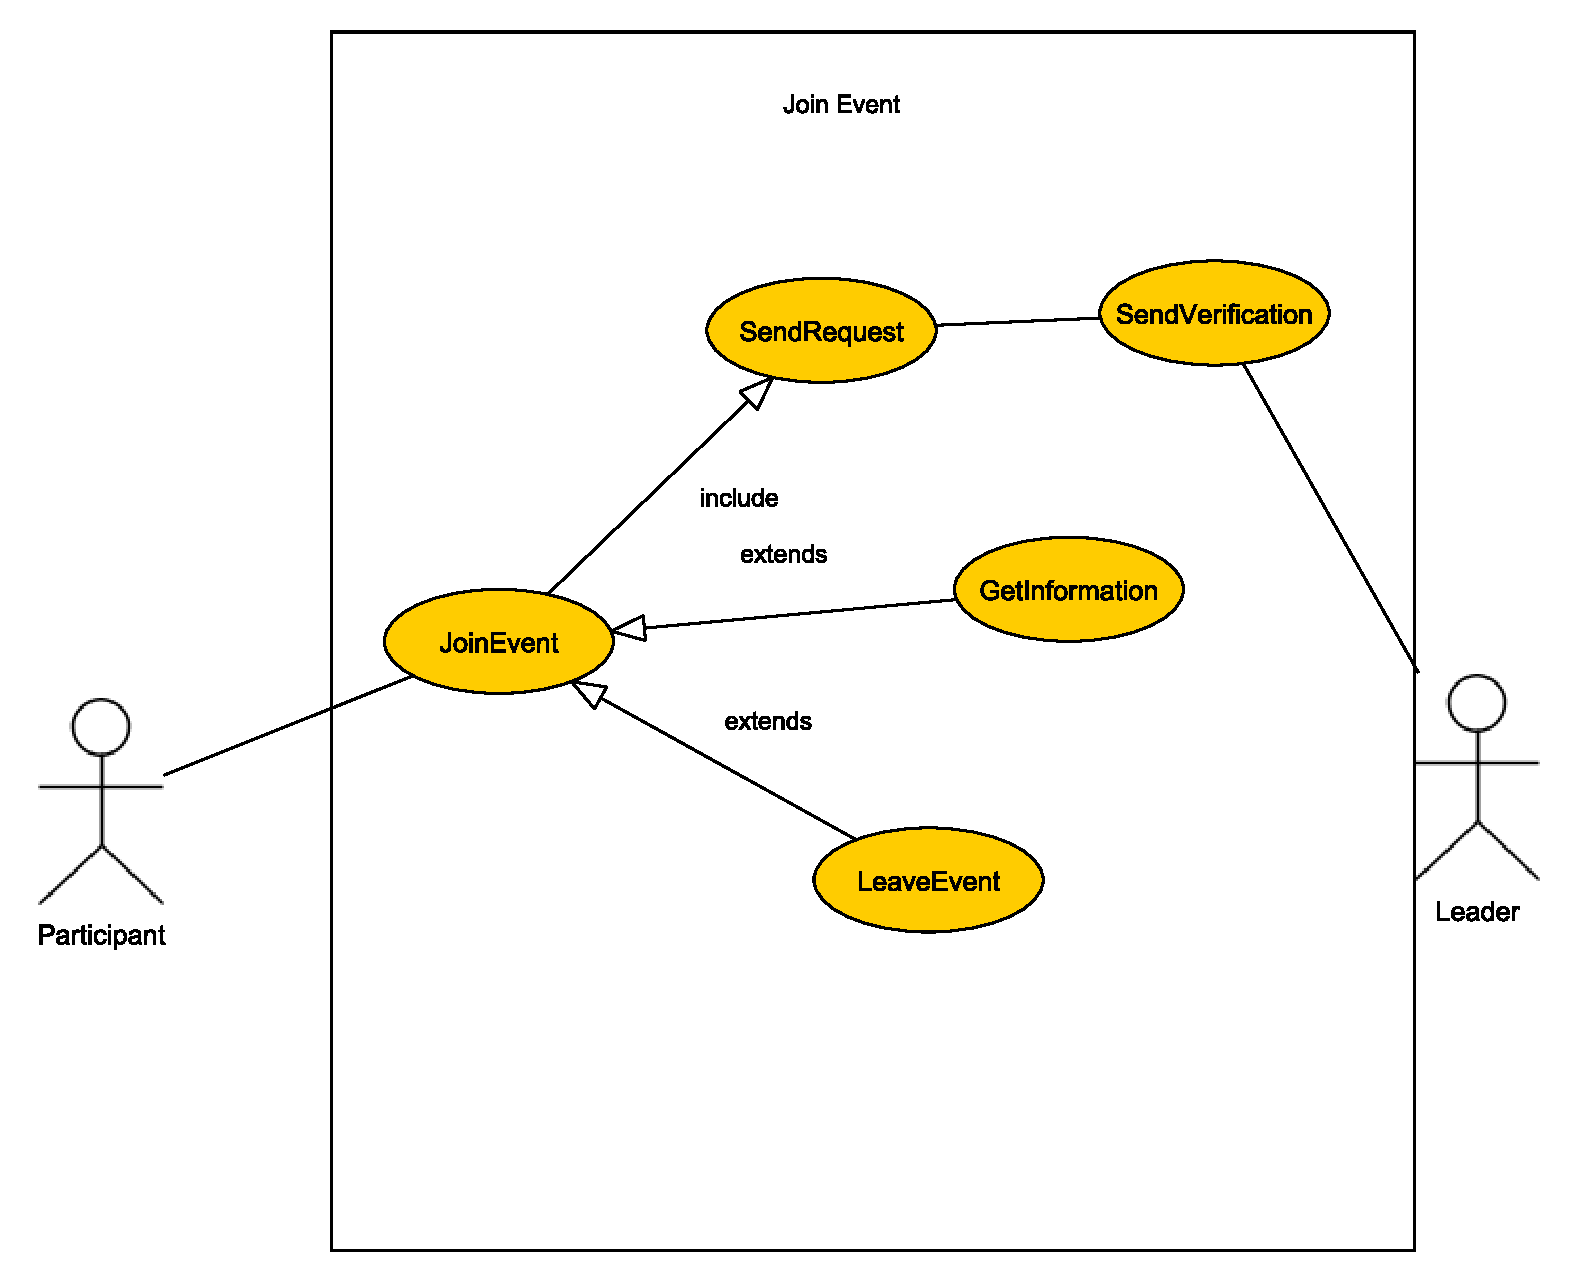
\includegraphics[scale=.5]{JoinEvent.png}

\subsection{Use Case Details}

\subsubsection{Characteristic Information}

\begin{tabular}{|l|l|}
\hline
Superior business process &  \\ \hline
Goal &  \\ \hline
Precondition &  \\ \hline
Postcondition &  \\ \hline
Involved User &  \\ \hline
Triggering Event &  \\ \hline
\end{tabular}

\subsubsection{GUI to call the use case}

\begin{tabular}{|l|l|}
\hline
Input field & Valid inputs \\ \hline
 &  \\ \hline
\end{tabular}

\subsubsection{Scenario for the standard use}

\begin{tabular}{|l|l|l|}
\hline
Step & User & Activity \\ \hline
 & & \\ \hline
\end{tabular}

\subsubsection{GUIs for the standard use}
\begin{tabular}{|l|l|}
\hline
Input field & Valid inputs \\ \hline
 &  \\ \hline
\end{tabular}
\subsubsection{Scenarios for non-standard uses}

\begin{tabular}{|l|l|l|}
\hline
Step & User & Activity \\ \hline
 & & \\ \hline
\end{tabular}

\subsubsection{GUIs for the non-standard uses}

\begin{tabular}{|l|l|}
\hline
Input field & Valid inputs \\ \hline
 &  \\ \hline
\end{tabular}

\subsubsection{Workflow}

\subsubsection{Open Points}

\pagebreak

\section{Non-functional Requirements}

\pagebreak

\section{Quantity Structure}

\pagebreak

\section{System Architecture and Interfaces}

\pagebreak

\section{Acceptance Criteria}

\pagebreak

\section{Acceptance Criteria}

\pagebreak

\section{References}

\pagebreak

\section{List of Figures}

\pagebreak

\end{document} 